%!TEX root = ../Main.tex


\chapter{Introduction}

%It defines the objectives and the importance of the research. It focus on the the application of Next Generation Sequencing to molecular biology, wheat genetics and ultimately to breeding programs. It also mentions the current status of the wheat reference genome and other resources (genetic maps, markers) the need of tools to query them effectively. 


\section{Wheat Genetics}
%The section describes alleles an the concept of gene, both as a locus in the genome (Quantitative Trait Locus, QTL) and an specific transcript (central dogma of molecular biology). Finally, it discuses traditional Mendelian inheritance and the effect of polyploidy.  Some of this is described in the Yr15 chapter, maybe it is not needed any more here. 


\subsection{Polyploidy and Wheat}
\label{lit:polyploidy}

A polyploid species contains more than one set of related genomes, that may come from a chromosomal duplication (autopolyploid) or from an hybridization with a related species (allopolyploid; \citealt{Shewry2009}) . 
\textit{Triticum aestivum} (bread wheat) has gone through an speciation event and two major hybridization events. 
Initially, a common progenitor evolved into two different species around 7 million years ago to form the A and B genomes, whose closest known relatives are \textit{Triticum urartu} and \textit{Aegelopolis speltoides}, respectively. 
At some point around 5.5 million years ago the D genome arouse, \textit{Aegilops tauschii}. 
Then, less than 800 thousand years ago the ancient A and B genome species hybridised and formed a tetraploid wheat, \textit{Triticum turgidum} ssp. \textit{dicoccoides} (wild emmer). 
A final event occurred less than 400 thousand years ago, when emmer wheat hybridized with \textit{Ae. tauschii}, leading to bread wheat (Figure \ref{lit:polyploidy}, \citealt{Marcussen2014}).  

\begin{figure}
  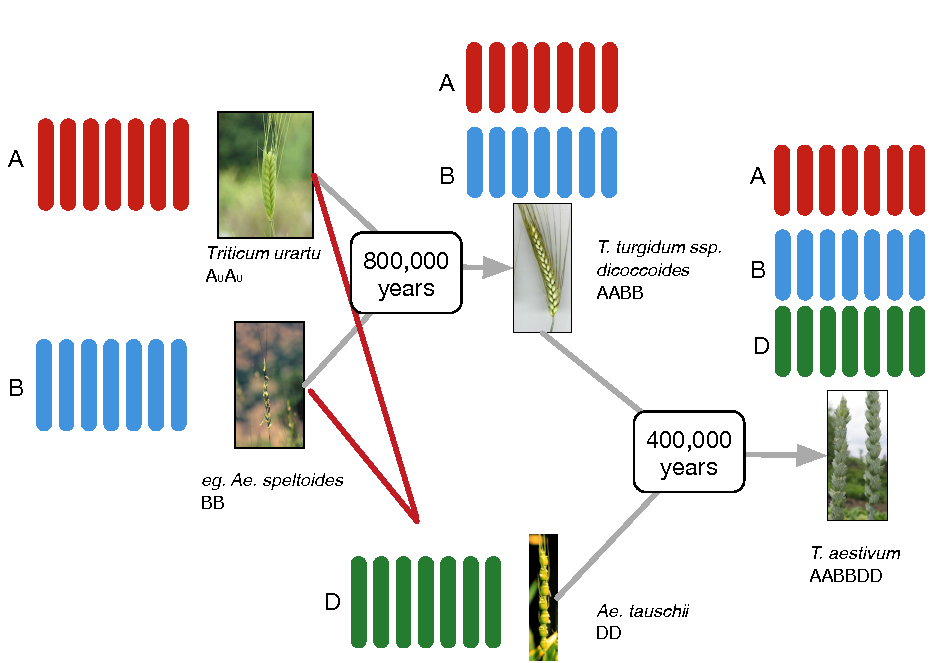
\includegraphics[width=1\textwidth]{LitReview/Figures/WheatPolyplodization.pdf}
  \caption{Hibridizations that lead to bread wheat \textit{T. aestivum}.  }
  \label{fig:lit:polyplody}
\end{figure}
Because bread wheat contains three related, yet independent copies of its genome, the expectation is that it has three copies of each genes, which are referred to as homoeologs. 

%\unsure{Talk about paralogues. }

%\subsection{Genetic Linkage}


\subsection{Experimental lines}

In crops, genetic research usually consists on crossing individuals and study the traits of the next generation. 
The progeny of a cross is called population. 
Groups of seeds with the same genetic background are called lines. 
Plants with the same homozygous background are pure lines. 
To study particular locus experimental lines are developed, the following list describe the most common \citep{VanOoijen2013Intro}:

\begin{description}
\item[F$_{1}$] The first generation of the cross between two plants. If the progenitors are different homozygous, all the population is heterozygous.  
\item[F$_{2}$ populations] come from a single heterozygous $F_{1}$ plant that is crossed to itself (self-crossed). The progeny is segregating (Fifure \ref{fig:lit:f2} with homozygous and heterozygous individuals. This type of population is used for the experiments in Chapter \ref{yr15} and it is described in more detail in Section \ref{yr15:f2}. 
\item[Back cross lones(BC)] are used to fix a trait on a genetic background. The process starts from a plant in the $F_{1}$ with the desired genotype or phenotype. This plant is crossed again to a plant from the line used as background ($P_{1}$). The progeny are called Back Cross 1 (BC1; Figure \ref{fig:lit:bc}). A plant from the BC1 with the desired genotype is selected and crossed to $P_{1}$. The process can be repeted, and with each cross the region linked to the target locus is narrowed. 
\item[Near Isogenic Lines (NIL)] After BC6, a line is considered Near Isogenic \citep{Stam1981}. At this level of back crossing most of the genetic material is the same as $P_{1}$, except for the region linked to the trait. 
\item[Recombinant Inbreed Lines (RIL)] are used to produce homozygous lines from an $F_{2}$ population. Each plant in the population is self-crossed. The lines that show an homozygous segregation are self-crossed again. After several iterations the line is considered homozygous. \ref{fig:lit:ri}).
\item[Double Haploid Lines (DH)] are an alternative technique to produce homozygous lines it. The individuals on the $F_{1}$ population are crossed to a different plant (ie maize crossed to produce wheat DH) to simulate pollination. On natural conditions, the gamets would be aborted. The embryos are rescued and treated with colchicine to induce a genome duplication. Since the duplication come from a single gamete, the resulting plant is homozygous (Figure \ref{fig:lit:dh}).

 
\end{description}

\begin{figure}
\centering
\begin{subfigure}{0.45\textwidth}
\centering
\caption{}
\label{fig:lit:f2}
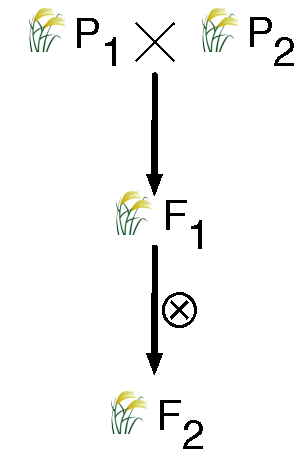
\includegraphics[height=0.20\textheight]{LitReview/Figures/crosses/F2.pdf}
\end{subfigure}
~
\begin{subfigure}{0.45\textwidth}
\centering
\caption{}
\label{fig:lit:bc}
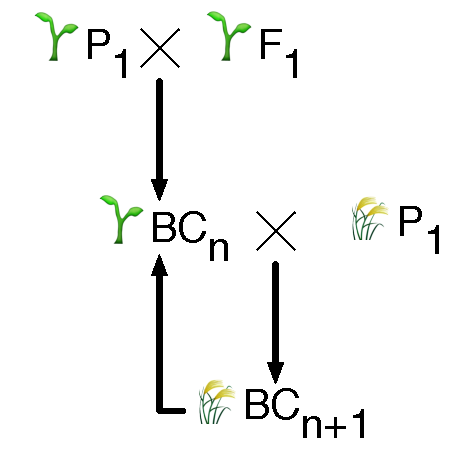
\includegraphics[height=0.20\textheight]{LitReview/Figures/crosses/BC.pdf}
\end{subfigure}


\begin{subfigure}{0.45\textwidth}
\centering
\caption{}
\label{fig:lit:ri}
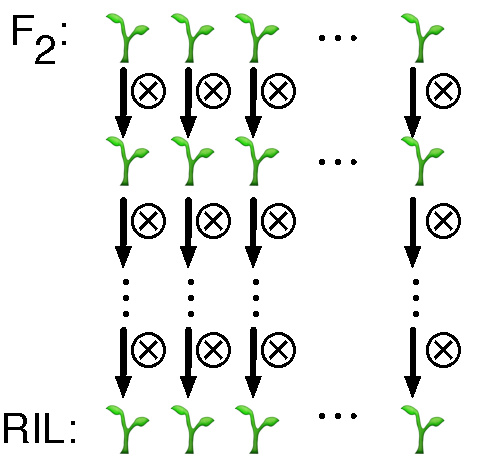
\includegraphics[height=0.20\textheight]{LitReview/Figures/crosses/RI.pdf}
\end{subfigure}
~
\begin{subfigure}{0.45\textwidth}
\centering
\caption{}
\label{fig:lit:dh}
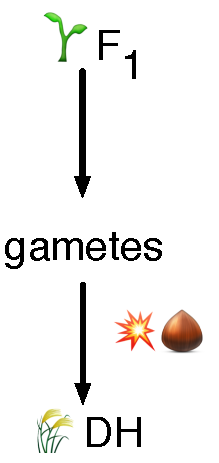
\includegraphics[height=0.20\textheight]{LitReview/Figures/crosses/DH.pdf}
\end{subfigure}

\caption[Types of experimental lines]{Types of experimental lines. 🌾 represent populations and 🌱 individual plants. ($\times$ represent a cross between lines. ($\otimes$) represent self-crosses. Ellipsis ($\ldots$) represent repetition. 💥🌰 represent a treatment to double the chromosomes from the gamete. (\subref{fig:lit:f2}) $F_{2}$ population. (\subref{fig:lit:bc}) Back Cross population. (\subref{fig:lit:ri}) Recombinant Inbred Lines. (\subref{fig:lit:dh}) Double haploid}
\end{figure}

%\subsection{Introgressions}

\section{Wheat Genomics}

\subsection{Molecular biology}
The genome is the genetic material of an organism, and can be studied using HTS to determine the sequence. 
However, only a small percentage of the genome is expressed in each cell in each condition, this differences in transcript production lead to differential gene expression between samples. 
The transcriptome is the complete set of RNA molecules present in a biological system during specific conditions\citep{wang2009rna}.  
The transcriptome of a sample and the differences in expression between samples can be studied using different methods. One of this is RNA-Seq, which is capable of capturing the dynamic range to quantify gene expression level\citep{Mortazavi2008}.

During transcription, a DNA sequence is transcribed into the primary RNA transcript (pre-mRNA) by the RNA polymerase. 
The RNA polymerase, and associated transcription factor, binds to promoter DNA and creates an RNA complementary copy. 
Depending on multiple factors, including gene regulation, this process can be repeated to create multiple copies of the sequence\citep{alberts2014molecular}.
The pre-mRNA suffers various modifications like splicing and capping. 
In a gene, there are  intragenic regions, called introns, that are removed from the pre-mRNA, while the remaining sequences, called exons, become part of the mature mRNA. 
Splicing is catalyzed by the spliceosome, which recognizes the sequences of the splice donor, branch and acceptor sites in the intron, cuts the intron and pastes the remaining exons.
In some cases, different introns and exons can be included or excluded, creating aternetive splicings of the RNA sequence\citep{alberts2014molecular}. 
Then, the 5' and 3' ends of the RNA sequence are modified to generate a mature messenger RNA (mRNA). 
A 7-methylguanosine cap is added to the 5' end. The 3' end is cleaved and polyadenidated, acquiring a poly(A) tail of approximately 200 adenines \citep{alberts2014molecular}. 
The result of this process is a mature mRNA, which forms part of the transcriptome.


\subsection{Primers and PCR}
To generate new copies of DNA, biological systems requiere a DNA polymerase to copy DNA into DNA or a reverse transcriptase to translate RNA to DNA. During DNA replication, the DNA polymerase binds to the template strand and to a short strand of RNA that serves as a primer for DNA synthesis and replication, and then adds complementary nucleotides. Eventually, this results in two complementary DNA strands\cite{alberts2014molecular}.

This process can be used to generate multiple copies of a DNA sequence using the \gls{pcr}. PCR uses an heat-stable DNA polymerase to amplify the template sequence. The DNA polymerase requieres a primer sequence that is complementary to the template strand to begin the reaction. Usually, chemically synthesized oligonucleotides of approximately 20 bases are added as primers. This primer sequence can be specific to the target region, or random if multiple regions are being duplicated. Once the DNA strand has been elongated, the temperature is elevated and then lowered to separate the DNA strands. The process is repeated multiple times to increase the number of DNA sequences exponentially\cite{alberts2014molecular}.


  
\section{Sequencing} 


\begin{figure}
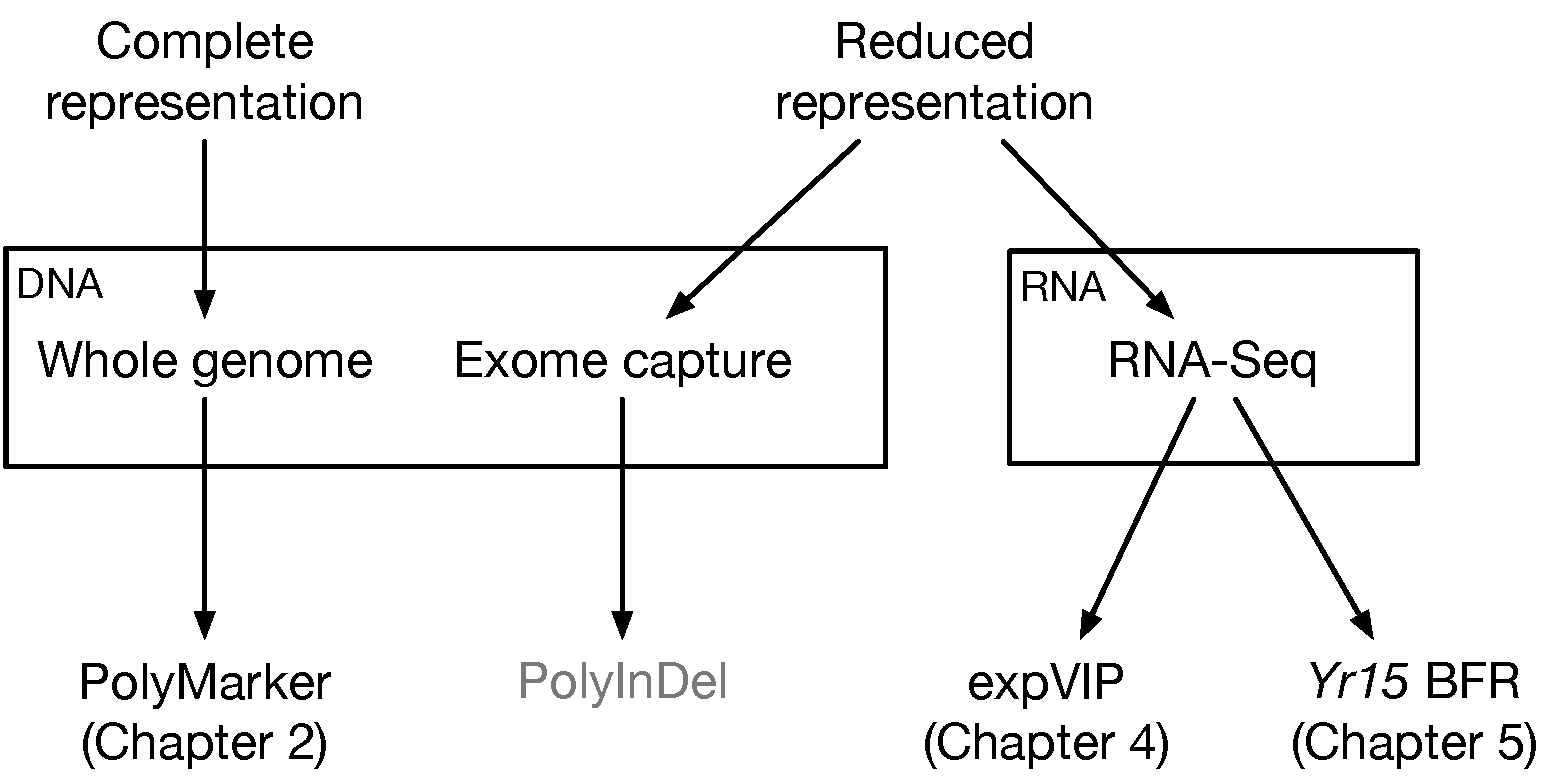
\includegraphics[width=1\textwidth]{LitReview/Figures/typesOfSequencing.pdf}
\caption{General types of sequencing ant their relationship with this PhD. PolyInDel is a project still in progress, not discussed in this Thesis. }
\end{figure}
\subsection{DNA sequencing with Illumina}

In the Illumina sequencer, the DNA library is loaded into a flow cell, where the fragments are captured by their adapters. 
Each fragment is amplified into clonal clusters, resulting in multiple copies of the sequence bounded to the surface in close proximity. 
Then, the sequencer detects the fluorescent dye-labelled oligonucleotides that are added one by one to the bound sequences by taking multiple images. 
This process can be repeated for each pair of the DNA. 
copies of the same sequence are clustered together, it is possible to analyse the images and detect which base is added to each cluster, determining multiple sequences with high fidelity, and exporting them as a FASTQ file \cite{RNAseqlopedia, truseq}.


According to the objectives of the experiment and the quality and volume of the available DNA, the library can be prepared on fragments of different sizes, the classification of the available sequencing for the fragments is the following \cite{Myllykangas2012,Metzker2010,Shendure2008,Hutchison2007}:

\begin{description}
\item[Single end] When the fragments are short, it is possible to just sequence from the 5'-end the read.
\item[Read Pairs] When the sample consists fragments of up to 500bp, it is possible to read the 5' end up to the read length were the quality starts to drop, the molecule can be turned upside down, reverse complemented and sequence backwards. It is not required, but ideally, the fragments sequenced with read pairs should be selected to have an homogenous size. The reads are in opposite orientation relative to each other. 
\item[Overlapping Read Pairs] are a variation to read pairs, where the size of the fragment is shorter than two times the read length. This allow an alignment between the two fragments to get an longer read with the limitations of the instrument.
\item[Mate pairs]  are used to get reads separated at distances between 1kbp and 5kbp. To achieve this, the molecule is circularised and the point were the two ends of the fragment were joint a biotin marker is inserted. Then, the molecule is fragmented again and the fragments containing the biotin are sequenced in the same fashion that read pairs. The resulting reads have the same orientation.
\end{description}


\subsection{RNA-Seq}
\label{lit:rna-seq}

%T is also possible to sequence the transcriptome of an organism. RNA-seq is a technology  where a set of mRNAs <ignoring other types> are sequenced to study the transcriptome of an organism. As current sequencing technologies, as Illumina, require a double-stranded complementary DNA (cDNA) template with  "adaptor" sequences and provide relatively short sequence reads (~75-250bp)\cite{} while  mRNAs are longer (gene models for wheat from \citealt{krasileva2013} are in a range between ~100 and 15,000bp), the RNA needs to be fragmented, converted to cDNA, and amplified so that the transcriptome can be analysed.

Both DNA and RNA can be sequenced using available HTS technologies
Originally, sequencers where designed with DNA in mind, so that analysing RNA requieres converting the transcriptome into a cDNA library\cite{RNAseqlopedia, truseq}.
To begin with, RNA is first isolated, purified and enriched for mature mRNA.  
For some sequencers, the resulting mRNAs need to be fragmented to improve sequence coverage, as current sequencers can only read sequences shorter than the transcripts. 
Once the quality of the RNA has been verified, it is converted into cDNA and adaptor sequences are added. 
First, the RNA strand is copied into first strand cDNA using the reverse transcriptase, as traditional polymerases cannot convert from RNA to DNA\cite{alberts2014molecular}.
Reverse transcriptase, as other polymerase, requires a primer annealed to begin the polimerization, so random primer are used to avoid 3' bias and improve coverage\cite{RNAseqlopedia, truseq}.
To obtain the second strand, RNase H is used to cleave the original RNA. 
The remaining fragments serve as primers for DNA polymerase I, creating a double-stranded complementary DNA. 
The cDNA fragments then go through an end repair process, the addition of a single ‘A’ base, and then ligation of the adapters, which will be used by the sequencer to read the sequence. 
The products are then purified, to remove artefact and their quality is verified\cite{RNAseqlopedia, truseq}.
The remaining sequences are enriched using the polymerase chain reaction (PCR),  which can generate thousands to millions of copies of a particular DNA sequence\cite{RNAseqlopedia, truseq}.
The resulting cDNA library is sequenced using available high throughput sequencing technologies. 
\unsure{Figure of This process}

\section{Sequence analysis}
%This section discusses the criteria to decide analysis done after sequencing, when to do re-alignments or \textit{de novo} assemblies, how to do SNP calling in diploid and polyploid organisims and the bulk frequency ratios.  

%DNA sequence alone is not alone to enough to understand the biology behind, a context is required. There are databases like Ensembl and NCBI that act as repositories of the known public sequences. 

From the computational point of view, the problem can be viewed as a string matching. The Smith-Waterman \cite{Smith1981} and Needleman-Wunsch\cite{Needleman1970} algorithms are the gold standard interns of accuracy looking for similarity between sequences. However, the execution time for both of them is prohibitive to run in massive databases. The algorithm execution time is O(mn), as it requires calculating a matrix of size $mn$ where $m$ is the target sequence and $n$ is the query sequence.  To scale this to a manageable problem algorithms like BLAST index the references and use heuristics to make the search more manageable, with some penalty in the accuracy. This alignments tools are useful for long stretches of DNA (like cDNA or contigs)\cite{Altschul1990}.

Several tools have been developed to do sequence alignment, among them the most common ones are:

\begin{description}
\item[BLAST] The BLAST heuristic algorithm compares a query sequence with those deposited in NCBI database, attempting to align the sections amongst them of significant sequence similarities \citep{Altschul1990}. BLAST is the most commonly used bioinformatics tool for sequence searching. When the query sequence and sequence within the database have a high sequence similarity and length coverage this is defined as a ‘hit’. The significant hits are generally termed as those that have protein sequence comparisons above 75\% sequence similarity and high coverage. BLAST accepts as input FASTA  or GenBank format of sequences.
\item[BLAT] Blast-Like Alignment Tool, is much faster than BLAST but less sensitive as it does a k-mer indexing of the database instead of a linear search, which means it finds seeds quicker. The way that BLAT performs quick analyses is by computing an "index of all non-overlapping K-mers in the genome". It is important to note that BLAT is less effective for sequences with less than 90\% sequence identity \citep{Kent2002}. This level of identity is enough to find the homoeologous genes in wheat, as they have an identity over 92\% between chromosomes \citep{Krasileva2013}
\item[Exonerate] Is another alignment program that works as a faster alternative to exhaustive sequence alignment methodologies, by implementing bounded sparse dynamic programming (BSDP).  It performs pairwise sequence comparisons, doing so by using various alignment models, exhaustive dynamic programming or different heuristic algorithms \citep{Slater2005}.  Exonerate is able to model intron-exon junctions when doing the alignment. 
\end{description}


When analysing high-throughput sequencing, having millions of short sequences make unfeasible to try to align the data to every possible reference. However, one can take in advantage the fact that you know which organism you are looking for and, if available, use a genomic reference. For this, tools like MAQ, BWA, Bowtie, among others, provide indexed search.  Once you have your reads aligned to a reference you can do more analysis, depending on the biological question being asked and the type of sequencing carried on.  Fortunately, most of the Short-Read sequence alignment produce similar outputs and the SAM format is becoming a de facto standard. This is allowing to make more modularised downstream analysis where you can test different aligners with different settings and pick the algorithm that better fits your experiment\cite{Liu2012,Li2009,Li2009a}. 

\subsubsection{\gls{iuapc} Ambiguity Codes}
\label{lit:ambiguity}
To represent polymorphisms in a single sequence the \gls{iuapc} has developed an representation of a single character combining more than one possible nucleotide. 
This table is used in Chapters \ref{cha:polymarker} and \ref{yr15} to represent \glspl{snp}.

\begin{table}
\caption{\gls{iuapc} ambiguity codes}
\centering
\begin{tabular}{ccc}
\toprule
IUPAC Code & Meaning & Complement \\
A & A & T \\
C & C & G \\
G & G & C \\
T/U & T & A \\
M & A or C & K \\
R & A or G & Y \\
W & A or T & W \\
S & C or G & S \\
Y & C or T & R \\
K & G or T & M \\
V & A or C or G & B \\
H & A or C or T & D \\
D & A or G or T & H \\
B & C or G or T & V \\
N & G or A or T or C & N \\
\bottomrule
\end{tabular}
\end{table}

\subsection{RNA-Seq}
\label{lit:RNASeq}

One way to narrow down which genes are involved in certain trait or response to the environment is to focus on studying only the expressed genes. One of the techniques involving \gls{ngs} is RNA-Seq. This technique captures the messenger RNA in the tissue being studied and sequenced. The premise is that you will find a gene more expressed if it is being used by the organism. Some proteins with a vital role for the cell are always expressed (i.e. RuBisCO for carbon fixation in plants\cite{CooperGM2000}). On the simplest of the experiments you would need two datasets to compare, one with the gene being looked expressed and one where it is not. The expression can come from different environmental conditions, development stage or different genotypes.\cite{Mortazavi2008} 

Depending on how much \textit{a priori} information of the analysed organism is available different bioinformatic approaches can be used.
\begin{description}
\item[Transcriptome alignment] The reads are aligned to a database of known cDNA. Ideally, alternative splicing sequences are available, so a simple alignment should work (i.e. BWA, bowtie). 
\item[Genomic alignment] The reads are aligned to the genome. The splice junctions, introns and axons need to be accounted, so simple alignment doesn't work. Regular alignments are used, but the reads may be trimmed at fixed sizes to allow discontinuous alignments using regular tools (i.e. Stampy, tophat/cufflinkns)
\item[\textit{De Novo} transcriptome assembly] If a reference of the organism is not available, it is possible to generate a draft transcriptome with the RNA-Seq reads with traditional assemblers (velvet, abyss) or with specialised assembler tools like Trinity. 
\end{description}

Once you have the alignments it is possible to evaluate the relative expression of the genes in the sample calculating the \gls{rpkm} or the \gls{tpm}. This normalises the expression by the amount of sequenced data and can be used to find which genes change in expression volume across different samples.   
%TODO: Write more details of RPKM vs TPM


\section{Wheat specific resources resources}
\label{lit:wheatResourcers}

During the course of this PhD, several resources were released in the wheat community. A timeline of the release of each one of those resource is in Figure \ref{fig:intro:timeline}. 

%\begin{landscape}
 \begin{sidewaysfigure}
  \centering
  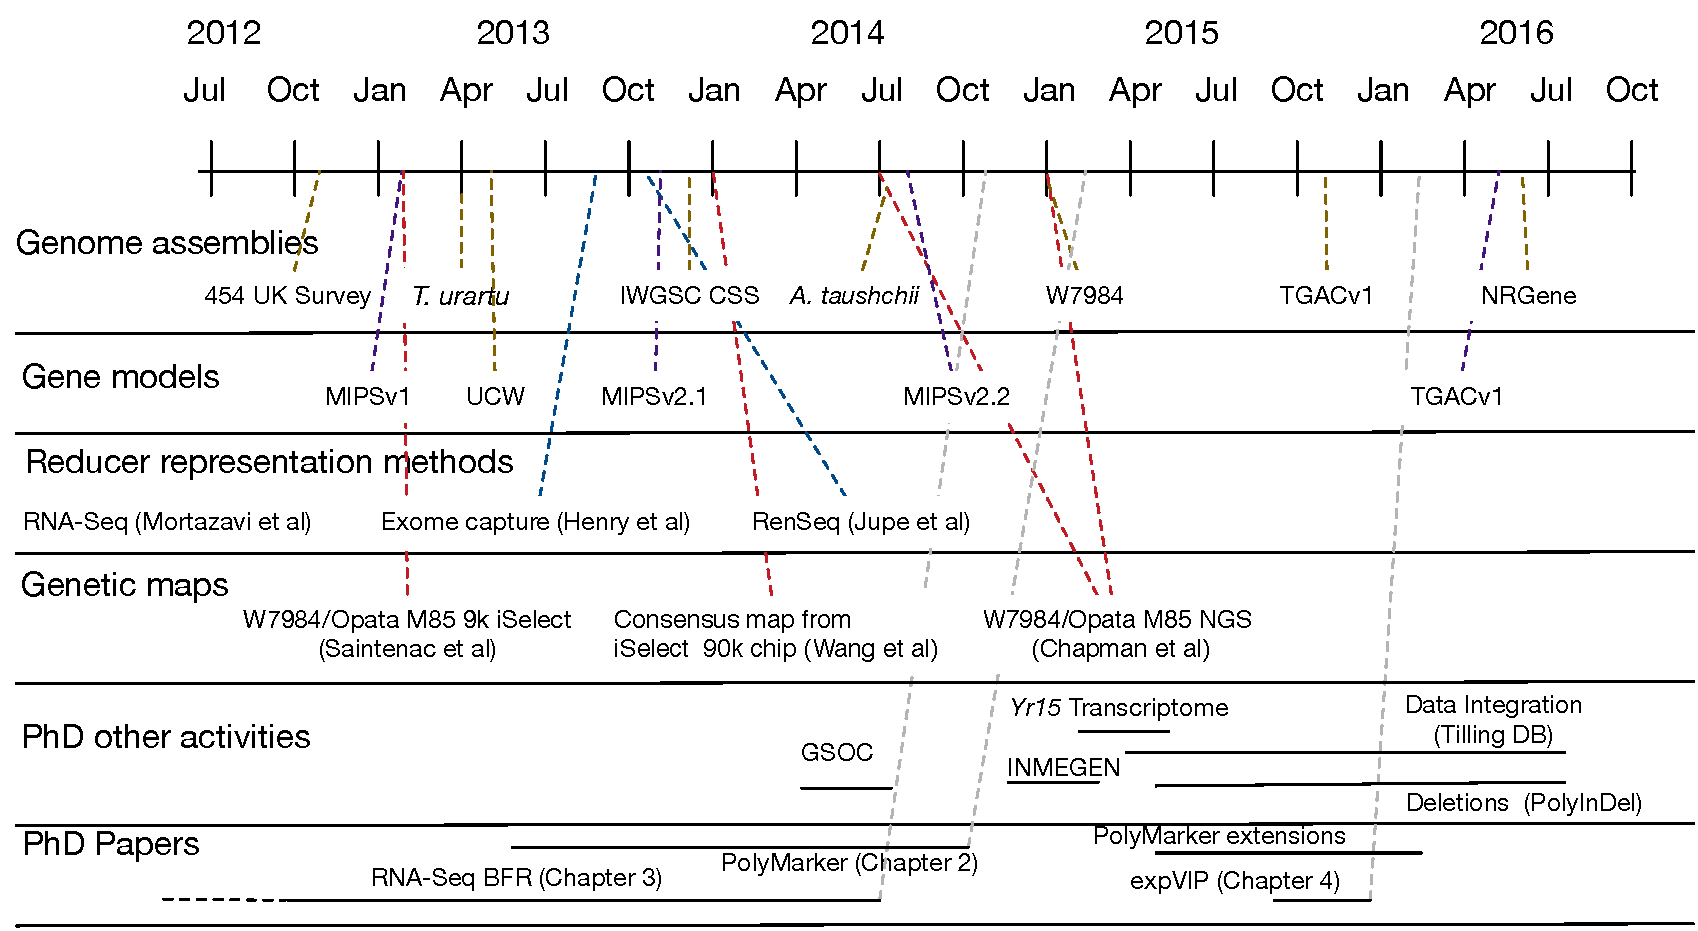
\includegraphics[width=1\textheight]{Introduction/RicardoPhdTimelineV1.pdf}
  \caption[PhD timeline.]{Timeline of the projects carried on during this PhD and the wheat resources that were released in the same period of time. }
  \label{fig:intro:timeline}
 \end{sidewaysfigure}
%\end{landscape}
\subsection{Genomic sequence}

The length of the genomic references available for wheat has been increasing year by year. During my PhD the following genomic references where published.   

\begin{description}
\item[454 Liverpool.] A \gls{wgs} sequencing project for \gls{cs} done in 454. The average coverage was around 5x. Assembling the reads produced an assembly with shorter contigs than the original reads. Hence, it was released as raw reads \citep{Brenchley2012}. Despite not being a proper reference genome, the reads where enough to find variations across the genomes and was used to designed genome specific primers before the IWGSC reference was published. 
\item[IWGSC CSS.] The \gls{iwgsc} is able to extract DNA from a single chromosome arm, using a method called flow sorting. DNA for each sample was sequenced with Illumina to a coverage of at least 60x and it was assembled \citep{Mayer2014}. The assembly is quite fragmented partly because the assembler not being able to cope with repetitive regions, and partly because the flow sorting reduces the quality of DNA, preventing the preparation of long fragments. 
\item[Chapman.] A \gls{wgs} project, but done with ilumina. Instead of sequencing \gls{cs}, a synthetic wheat was used. The scaffolds are longer than the \gls{css} assembly, but the project was not annotated. It was used mainly to develop markers in a mapping population between synthetic (W7984) and non-synthetic (Opata) wheat lines \citep{Chapman2015}.   
\item[TGACv1] A \gls{wgs} originally proposed as an improvment to the \gls{css} assembly. The scaffolds are longer than in Chapman and it uses the contigs from \gls{css} to assign the chromosome arm corresponding to each contig. An annotation for this assembly is available \citep{Clark2016}
\end{description}


\subsection{Gene models}

For this thesis, a set of gene models correspond to the coding sequence of a gene. 
The following sets of gene models are used in this thesis. 

\begin{description}
\item[UniGenes.] This is an effort of the \gls{ncbi} to unify several \acrshortpl{est} deposited on their databases, per species.
The set is generated automatically by aligning all the ESTs to each other and clustering them by identity. 
The longest EST is selected as the canonical representation of the gene \citep{PontiusJUWagnerL2002}. 
Because this approach is not aware of the different genomes, and the set of ESTs may not include them, the algorithm  collapses homoeologous genes. 
This needs to be taken in account when doing down stream analysis. 
\item[\acrshort{ucw} gene models.] This set of gene models come for tetraploid wheat come from a \textit{de novo} assembly of \textit{T. turgidum} (AABB) a \textit{T. urartu}. 
In both cases RNA-Seq was assembled with several parameters and the resulting assemblies where merged. 
To separate homoeologues genes that were assembled as a single gene, the reads were aligned to the assembly.
Then, the phasing of the reads was used to separate the gene in the two homoeologues \citep{Krasileva2013}.
This gene models are useful for tetraploid wheat. 
When using this reference with hexaploid wheat, care must be taken of reads coming from the D genome that will map to one of the alternative homoeologues. 
\item[Genome annotation IWGSC.] To complement the \acrshort{css} genome assembly, the genome was annotated using related grasses ( \textit{Brachypodium distachyon}, \textit{Oryza sativa}, \textit{Sorghum bicolor}, and \textit{Hordeum vulgare}. 
The annotation was supported by RNA-Seq data from five samples from different tissues at three developmental stages \citep{Mayer2014}. 
This was the first genome-scale annotation effort including the three genomes independently. 
The main caveat of this annotation is that due the relatively small size of the scaffolds used as reference, several genes are split in two different gene models. 
\item[Genome annotation TGACv1.] This is the companion annotatuin for the TGACv1 assembly. 
The annotation was produced with a novel approach, by merging four alternative assemblies from three RNA-Seq datasets. 
Also, long reads from PacBio where used to validate the gene models (ie. Full length, alternative splicing, canonical sequence) \citep{Venturini2016}. 
This gene models were made public during the last year of this PhD, hence they were not used for the analysis. 
However the tools described in Chapters \ref{cha:polymarker} and \ref{cha:exp} can work with the updated gene models. 
\end{description}



\subsection{Genetic markers and maps}

The development of high resolution genetic maps had been benefited by technologies like SNP arrays and \gls{ngs}. 
\gls{snp} arrays allow the genotyping of thousands of alleles from a single plant. Likewise, low coverage sequencing can be used with the support of a good reference to do genotyping. 
Both techniques had been used recently to produce the following genetic maps: 

\begin{description}
\item[90k iSelect chip] This dataset consist of 81,597 \glspl{snp} coming from 19 hexaploid and 18 tetraploid wheat accessions and, a an aggregation of previously published SNPs. The wheat accession where sequenced with RNA-Seq and the reads where used to detect polymorphisms. The sequence flanking the SNPs come may include the intron-exon junction. 46,977 of the SNPs were genetically mapped with a combination of eight mapping populations \citep{Wang2014}. 
\item[820k Axiom chip] The \gls{snp} discovery for this array was done using exome capture from 43 bread wheat and relative species. Three mapping populations (Avalon $\times$ Cadenza, W7984 $\times$ Opata and Savannah $\times$  Rialto) were used to prduce a consensus map with 56,505 markers \citep{Allen2016,Winfield2016}. This points out that a higher number of markers does not necessarily means a higher resolution in the genetic map, the main constrain are the mapping populations.  
\item[Popseq/Chapman] The SNPs came from a mapping population of 90 individuals, all consisiting of \gls{dh} lines from a cross W7984 $\times$ Opata. Those \gls{dh} lines were lightly sequenced, with a coverage less than 2$\times$. Because of the high density of the SNPs, the haplotypes could be inferred. The total number of SNP is over 24 million, but the minimal set of markers 112,687 for the genetic map. The same population was used for the original \gls{css} assembly \citep{Mayer2014} and the assembly from \citet{Chapman2015}. 
\end{description}


%\subsection{Online resources}
%Portal
%-CeralsDB
%-MASWheat
%-Ensembl
%-Wheat-expression
%-Copo

%The Collaborative Open Plant Omics (COPO; \citealt{Davey2015}) is a an initiative to integrate data from different databases. 
%The idea is to improve the interaction across repositories through an \gls{api}, a standard way to ensure the interoperability between systems. 
%This approach keeps the responsibility of the system and data maintenance on the service providers. 
%Service providers must ensure the compliance to standard of curation and integration, which would simplify the data analysis and visualisation, and ultimately promote the use of the integrated resources.  


\section{Aim and objectives}


The main aim of this PhD is to develop bioinformatics tools that help answer biological questions of importance by addressing the complexities associated with the wheat genome, such as its size and polyploid nature. 
These tools can only be effective if they are designed within a biological context and as such I have worked alongside experimental biologists over the past four years. 
The strategies and resources developed in this PhD take advantage of the latest developments in wheat research and I incorporated these as they were made public (Figure \ref{fig:intro:timeline}). 
The topics covered by this thesis, their relationship and, the chapter where they are used are shown in Figure \ref{fig:intr:topics}.

As my aim was to develop new approaches, strategies and tools in polyploid wheat, I have listed a series of objectives, rather than specific hypotheses, which I tried to address over the course of this PhD. 


\begin{enumerate}

\item Simplify and automate the design of primers for marker assisted selection in polyploid wheat (Chapter \ref{cha:polymarker}).
\item Develop a pipeline that can be used to find genetic markers for breeding, using bulked segregant analysis and reduced representation sequencing  (Chapter \ref{yr15}).
\item Develop a platform to integrate and visualize RNA-seq expression experiments (Chapter \ref{cha:exp})
\item Establish an overall framework to integrate the different resources developed in this PhD (Chapter \ref{cha:discussion}).
\end{enumerate}

\begin{figure}
\centering
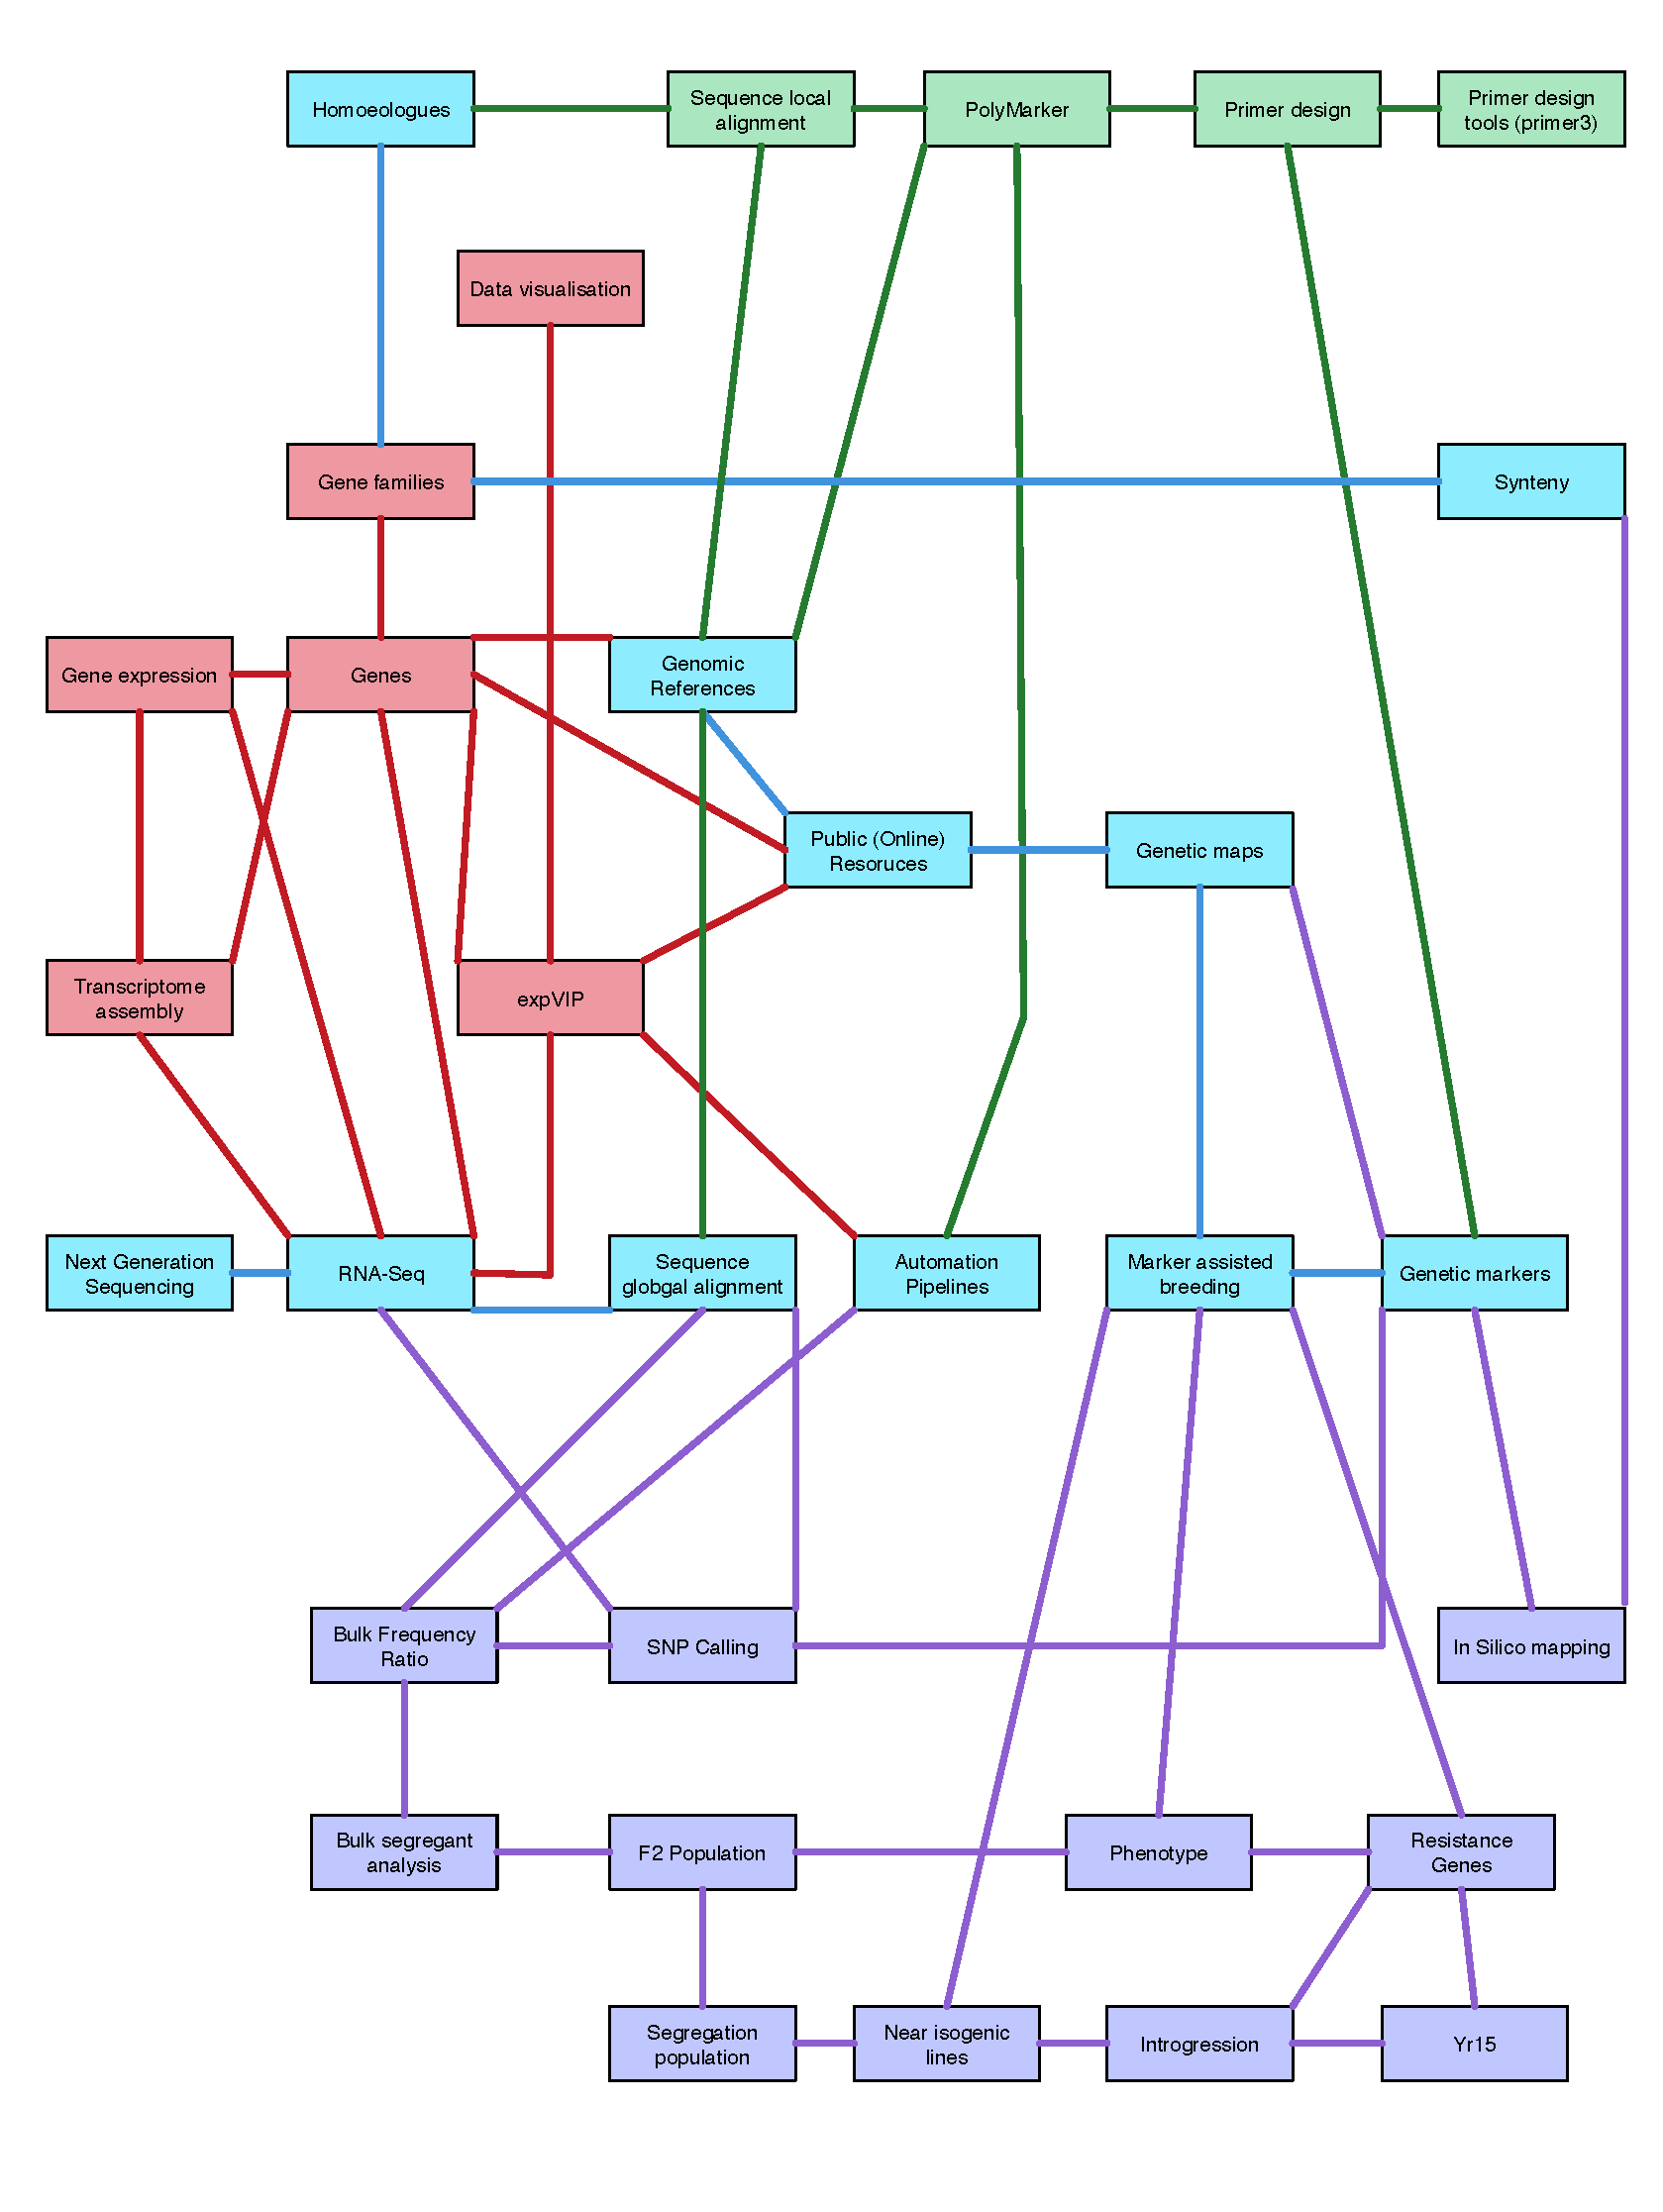
\includegraphics[width=1\textwidth]{Introduction/RicardoThesisTopics.pdf}
\caption{Topics of this Thesis}
\label{fig:intr:topics}
\end{figure}


All the pipelines and data produced by this project are publicly available. Towards this end I have also strived to publish this research in open access journals. Peer reviewed publications stemming from these research chapters are listed below: 

\begin{itemize}
\item Chapter 2 (PolyMarker)
\begin{itemize}
	\item \textbf{Ramirez-Gonzalez RH}, Uauy C, Caccamo M (2015) PolyMarker: a fast polyploid primer design pipeline. Bioinformatics, doi:10.1093/bioinformatics/btv069 (corresponding author)
	\item King R, Bird N, \textbf{Ramirez-Gonzalez RH}, Coghill JA, Patil A, Hassani-Pak K, Uauy C, Phillips AL (2015) Mutation scanning in wheat by exon capture and next-generation sequencing. PlosOne. 10 (9), e0137549
	\item Hubbard A, Lewis CM, Yoshida K, \textbf{\textbf{Ramirez-Gonzalez RH}}, de Vallavieille-Pope C, Thomas J, Kamoun S, Bayles R, Uauy C, Saunders DGO (2015) Field pathogenomics reveals the emergence of a diverse wheat yellow rust population. Genome Biology 16:23 
\end{itemize}

 \item Chapter 3 (Bulked segregant mapping)
\begin{itemize}
\item	\textbf{Ramirez-Gonzalez RH}, Segovia V, Bird N, Fenwick P, Holdgate S, Berry S, Jack P, Caccamo M, Uauy C (2014) RNA-Seq bulked segregant analysis enables the identification of high-resolution genetic markers for breeding in hexaploid wheat Plant Biotechnology Journal 13:613-624
\item	\textbf{Ramirez-Gonzalez RH}, Segovia V, Bird N, Caccamo M, Uauy C (2015) Next Generation Sequencing Enabled Genetics in Hexaploid Wheat. in Advances in Wheat Genetics: From Genome to Field eds Ogihara Y, Takumi S, Handa H, pg 201-209
\end{itemize}
\item Chapter 4 (expVIP)
\begin{itemize}
	\item Borrill P, \textbf{Ramirez-Gonzalez RH}, Uauy C. 2016. expVIP: a customisable RNA-Seq data analysis and visualisation platform. Plant Physiology 170:2172 (joint first author) 
\end{itemize}
\end{itemize}





